\chapter{Experimental Uncertainties}


\section{Introduction}

In this lab, you will explore how the sample mean and sample variance
can be used to estimate experimental uncertainties.  You will also use
the Monte Carlo method to explore the standard propogation of
uncertainties to calculated quantities.

\section{Sample Mean and Sample Variance}

The Monte Carlo simulation of experimental data is an essential tool of
experimental physics in large part because, unlike in our real
experiments, we know the true values of the parameters used to produce
our simulated experimental data.

In this section, we will use the Monte Carlo method to examine the
statistical properites of the sample mean and sample variance, from a
series of experiments each making repeated measurement of a single
quanity $x$.  We'll produce our simulated experiments with known
parameters $\mu$ and $\sigma$, which are the ``true values'' of the
simulation.  We'll then calculate experimental estimates for these
quantities and compare them to the known true values.

\begin{figure}[htbp]
\begin{center}
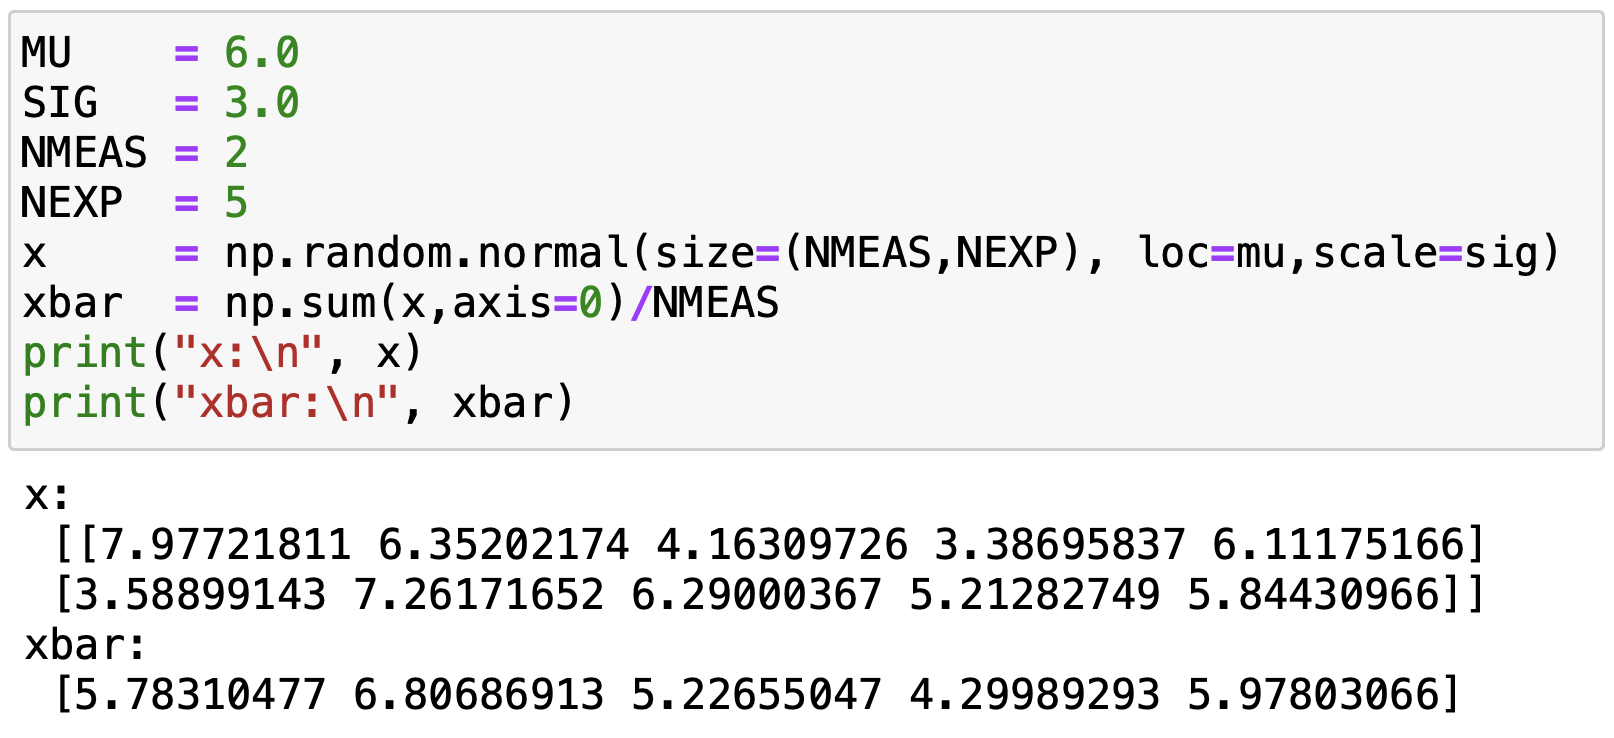
\includegraphics[width=0.75\textwidth]{figs/uncertainties/pseudoexps-code.png}\\
\end{center}
\caption{\label{fig:pseudoexps} Five simulated experiments each averaging two measurements.}
\end{figure}

As we will need to simulate multiple experiments, and each experiment will
make multiple measurements, our simulated measurements will be in the
form of a 2-D numpy array, as showin in Fig.~\ref{fig:pseudoexps}.
When looking through the example, note the following key features:

\begin{itemize}
\item There are two counts to consider, the number of experiments {\tt
  NEXP} and the number of measurements {\tt NMEAS}.  For example, if
  we want to study the statistics of experiments involving only a few
  measurements, we can still simulate many experiments, each with only
  a few measurements.

\item We simulate measurements by throwing random numbers from a
  Gaussian distribution, using the function {\tt np.random.normal}.
  The argument {\tt loc} is the mean and the argument {\tt scale} is
  $\sigma$.

\item We compute sums using the {\tt np.sum} and use the argument {\tt
  axis} to sum the columns.  After summing the columns in our {\tt
  NMEAS}x{\tt NEXP} matrix, we are left with a 1-D array with one sum
  per experiment.
  
\item Notice that there are no for loops.  The C++ version of this code
  would use two.  It might take some getting used to, but this is one
  of the features that makes Python less error prone and more fun to
  write.  You spend less time on boring bookkeeping of counts and more
  time thinking about the problem itself.
\end{itemize}

An experiment with $N$ measurements of a quantity $x$ can estimate any
$\braket{f(x)}$ as:
\begin{displaymath}
\bar{f} = \frac{1}{N} \sum_i f(x_i)
\end{displaymath}
This is because the measurements $x$ are drawn from the distribution $P(x)$ associated with the experiment and so the sum is an approximation for the integral:
\begin{displaymath}
\braket{f(x)} = \int f(x_i) P(x) dx
\end{displaymath}
This is why $\bar{x}$ is a good experimental estimate for
$\mu$.  We can use the same technique to estimate the experimental
uncertainty $\sigma$ as the standard deviation of the measured values.
While the variance is defined as:
\begin{displaymath}
\sigma^2 = \braket{(x-\mu)^2} = (x -\mu)^2 P(x) dx
\end{displaymath}
we can estimate it from the data as:
\begin{displaymath}
\sigma^2_\mu = \frac{1}{N } \sum_i (x_i -\mu)^2 
\end{displaymath}
provided that we know the true value of $\mu$, which we do in this case.  We'll call this quantity
the sample variance with respect to $\mu$.  When using Monte Carlo simulation, it is often illuminating to use ``truth'' information, as we do here, but keep in mind that there is no corresponding experimental technique!

\begin{plot}\end{plot}
Simulate 100,000 experiments each making 10 measurements of a value
$x$, drawn from a Gaussian distribution with $\mu=5$ and $\sigma=2$.
Use the summing technique (along an axis) to calculate the sample
variance with respect to $\mu$:
\begin{displaymath}
\sigma^2_\mu = \frac{1}{N } \sum_i (x_i -\mu)^2 
\end{displaymath}
Make certain to use the true value $\mu=5$.  As always, start with a
small numbers (e.g, 10 experiments each making 3 measurements) while
developing and debugging your code.  Then scale up to the requested
numbers once your code is working reliably.  Calculate the ratio of
$\sigma^2_\mu$ to the true value $\sigma^2 = 4$.

Calculating the sample variance with respect to $\mu$ requires knowing
the true value of $\mu$.  This situation does sometimes arise in the
lab, such as when you are calibrating your device with a known input.
In this case, you know the true value $\mu$, and you can estimate the
uncertainty of your measurement $\sigma$ by calculating $\sigma_\mu$.

Often, however, the entire purpose of your experiment is to measure
the unknown quantity $\mu$.  Supposing one did not know the
uncertainty of the measurement $\sigma$, how could you obtain an
estimate.  The best you can do, in this case, is use your best
estimate of $\mu$ which is $\bar{x}$ and calculate
\begin{displaymath}
s_N^2  = \frac{1}{N} \sum_i (x_i-\bar{x})^2.
\end{displaymath}
The quantity $s_N^2$ is called the sample variance, and the quantity
$s_N$ is called the sample standard deviation.

\begin{plot}\end{plot}
Modify your code to calculate the sample variance:
\begin{displaymath}
s_N^2  = \frac{1}{N} \sum_i (x_i-\bar{x})^2.
\end{displaymath}
Use the {\tt np.sum} function as in the previous exercise.  Calculate the ratio of $s^2_n$ to the true value $\sigma^2 = 4$.

You results should show that for $N=10$ the sample variance $s^2_N$ is
biased from the true value of $\sigma^2$.  It turns out that
\begin{equation}
\braket{s_N^2} = \frac{N-1}{N} \sigma^2
\end{equation}
which is an optional exercise in the lecture notes.  A plausible
explanation for this effect comes from noting that the quantity:
\begin{displaymath}
\sum_i (x_i - \mu) 
\end{displaymath}
is unknown whereas our definition of $\bar{x}$ implies that
\begin{displaymath}
\sum_i (x_i - \bar{x}) = 0
\end{displaymath}
Which is a fixed constraint on the $N$ values used to compute the sum in
$s_N^2$.  This constraint reduces the number of independent
measurements to $N-1$, biasing the result by the factor $(N-1)/N$.

Understanding this bias allows us to caculate the {\em unbiased} sample variance as:
\begin{displaymath}
s^2 = \frac{1}{N-1}\sum_i (x_i - \bar{x})^2 
\end{displaymath}
The use of $N-1$ instead of $N$ is called Bessel's correction.

\begin{plot}\end{plot}
Modify your code to calculate the unbiased sample variance:
\begin{displaymath}
s^2  = \frac{1}{N-1} \sum_i (x_i-\bar{x})^2.
\end{displaymath}
Use the {\tt np.sum} function as in the previous exercise.  Calculate the ratio of $s^2_n$ to the true value $\sigma^2 = 4$.

Numpy provides the functions {\tt np.mean} and {\tt np.var} to
calculate the sample mean and sample variance.  You can use the
argument {\tt ddof} to select between the biased and unbiased sample
variation.

\begin{plot}\end{plot}
Modify your code to calculate mean, biased sample variance and
unbiased sample variance, using the numpy functions {\tt np.mean} and
{\tt np.var}.
  
\begin{figure}[htbp]
\begin{center}
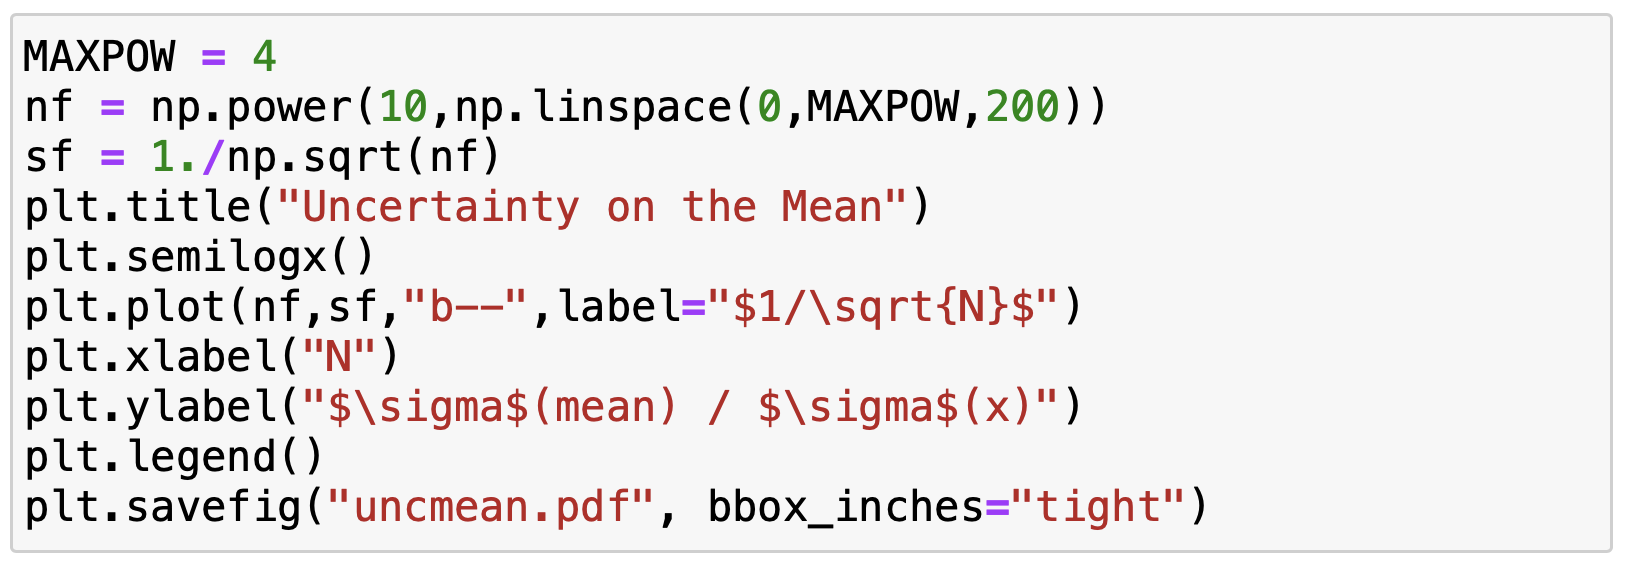
\includegraphics[width=0.75\textwidth]{figs/uncertainties/uncmean-code.png}\\
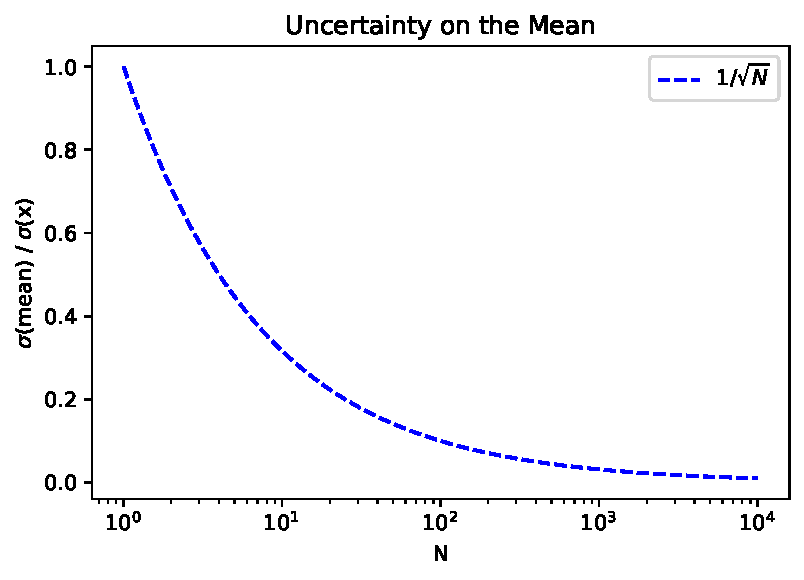
\includegraphics[width=0.75\textwidth]{figs/uncertainties/uncmean.pdf}\\
\end{center}
\caption{\label{fig:uncmean} The uncertainty on the mean versus number of measurements.}
\end{figure}

We showed in lecture that the uncertainty on the sample mean $\bar{x}$ of $N$ measured values is smaller than the uncertainty $sigma_x$ of the individual measurements:
\begin{displaymath}
\sigma(\bar{x}) = \sigma_x / \sqrt{N}
\end{displaymath}
This relationship illustrated in Fig.~ref{fig:uncmean}. When looking through the example code, notice the following features:
\begin{itemize}
\item The x-axis is plotted on a log scale, by the function call {\tt plt.semilogx}
\item If the $x$ values {\tt nf} for plotting a smooth function where
  choosen uniformly in N, there would be roughly 10,000 times as many
  points above $N=10^3$ as below $N=10^1$.  To make the plot smooth
  everywhere would require a {\em lot} of points.  Instead, the
  $x$-axis values are determined as $N = 10^a$ where $a$ is chosen
  uniformly in the range $[0,4]$.  This is a very useful technique!
\end{itemize}

\begin{plot}\end{plot}
Simulate 10,000 experiments each of which make $N$ measures of a
quantity $x$ with $\mu=0$ and $\sigma=1$.  Calculate the unbiased
sample variance of each experiment, and then the mean of these sample
variances across all experiments.  Plot the results as function of $N$
for $N=1,10,10^2,10^3$ and $10^4$.  On the same axis, included the
prediciton from Fig.~\ref{fig:uncmean}.


\begin{plot}\end{plot}
Modify your previous example so that {\em both} the $x$-axis and
$y$-axis have a log scale.  Why does the function now appear linear?

\section{Propagation of Uncertainties}

\begin{figure}[htbp]
\begin{center}
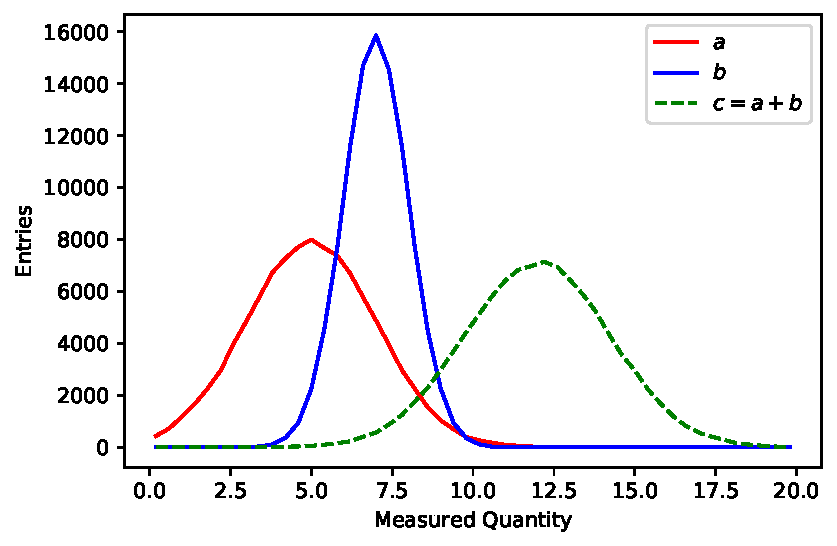
\includegraphics[width=0.75\textwidth]{figs/uncertainties/addunc.pdf}\\
\end{center}
\caption{\label{fig:addunc} Simulation of many measurements of the quantity $c = a + b$. }
\end{figure}

Consider two measured values $a \pm \sigma_a$ and $b \pm \sigma_b$.  If we calculate the quantity $c = a + b$ or $c = a - b$, the uncertainty on the calculated value $c$ is given by:
\begin{displaymath}
\sigma_c = \sqrt{\sigma_a^2 + \sigma_b^2}.
\end{displaymath}
If instead, we calculate $c = a \cdot b$ or $c = a/b$ the fractional uncertainty on $c$ is given by:
\begin{displaymath}
\frac{\sigma_c}{c} = \sqrt{\left(\frac{\sigma_a}{a}\right)^2 + \left(\frac{\sigma_b}{b}\right)^2}.
\end{displaymath}
In this section, you'll develop a numerical simulation for the
propagation of uncertainties under addition, subtraction,
multiplication, and division.  An example, for $c = a + b$ is shown in Fig.~\ref{fig:addunc}.

\begin{plot} \end{plot}
Simulate the measurement $a$ by drawing 100,000 random samples from a
Gaussian distribution with mean $a$ and sigma $\sigma_a$, and do
likewise for $b$.  Calculate the values $c = a -b $ from the $a$ and
$b$ values.  Plot the distribution of all three variables (as in
Fig.~\ref{fig:addunc}) as histograms with 50 bins and an appropriate
range.  Use values of $a$ and $b$ that are different from the example.
Calculate the mean and variance of the simulated $c$ values
and compare to your expectations from the standard propagation of
uncertainties.

\begin{plot}
Repeat the previous exercise but for multiplication.  Use new values
for $a$ and $b$ if you like.
\end{plot}

Our general formula for propogating uncertainties uses a Taylor
explansion approximation.  This means that the approximation is not
valid if the function is varying wildly within the variable
uncertainties.  This condition can be easily broken for division
$a/b$.

\begin{plot}
Repeat the previous exercise but for division.  Find values
for $a$ and $b$ which cause the standard propogation of uncertainty to fail.  What should an experimenter do in such case.  (Hint:  you are looking at it!)
\end{plot}




























